%%
%% (
%%  )\ )                             (
%%  (()/(   (            (             )\  )   (
%%   /(_))  ))\   (       ))\  (   (   (()/(   ))\
%%   (_))  /((_)  )\  )  /((_) )\  )\   ((_))/((_)
%%   | _ \(_))(  _(_/( (_) )  ((_)((_)  _| |(_))
%%   |   /| || || ' \))/ -_)/ _|/ _ \/ _` |/ -_)
%%   |_|_\ \_,_||_||_| \___|\__|\___/\__,_|\___|
%%

\documentclass{article}
\usepackage[utf8]{inputenc}
\usepackage[spanish]{babel}
\usepackage{amsmath}
\usepackage{amsfonts}
\usepackage{amssymb}
\usepackage{graphicx} % Paquete para incluir imágenes en el documento LaTeX
\usepackage{subfigure}
\usepackage{hyperref}
\hypersetup{
  colorlinks=true,
  linkcolor=blue,
  filecolor=magenta,
  urlcolor=cyan,
}
\urlstyle{same}
\usepackage{varwidth}

\newcommand\tab[1][1cm]{\hspace*{#1}}

\usepackage{multirow}

\usepackage[a4paper,rmargin=1.5cm,lmargin=1.5cm,top=1.5cm,bottom=1.5cm]{geometry}

\usepackage{pdfpages}

\usepackage{xcolor}
\usepackage{minted}
\usemintedstyle[cpp]{monokai}
\usemintedstyle[python]{paraiso-dark}
\usemintedstyle[bash]{manni}
\usemintedstyle[bat]{colorful}
\definecolor{LightGray}{gray}{0.9}
\definecolor{DarkGray}{gray}{0.1}
\definecolor{MidGray}{gray}{0.8}
\definecolor{codegreen}{rgb}{0,0.6,0}
\definecolor{codegray}{rgb}{0.5,0.5,0.5}
\definecolor{codepurple}{rgb}{0.58,0,0.82}
\definecolor{backcolour}{rgb}{0.95,0.95,0.92}

\setlength{\parindent}{0px}  % Setea la indentacion de la primera linea de cada parrafo a cero pixeles.


\title{Un titulo}
\author{@RuneCode}

\begin{document}
%% Portada
\includepdf{./portada/portada.pdf}

\section{Instalación de Git}%
La instalación de este controlador de versiones es importante porque nos
permitirá gestionar el avance de nuestros proyectos.\\

Su instalación es sencilla, tan solo se tiene que visitar su
\href{https://git-scm.com/}{página web} y seleccionar la opción
\textbf{Download for Windows} tal y como observamos en la siguiente imágen...

\begin{figure}[h!]
  \centering
  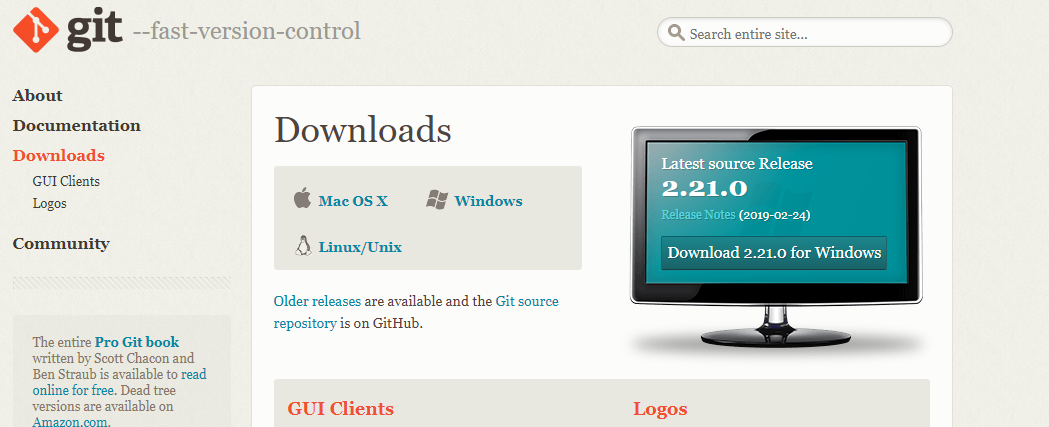
\includegraphics[scale=0.5]{./imagenes/Gitbash.png}
\end{figure}

Luego de descargar el instalador se debe ejecutar como administrador, es recomendable seguir
la instalación con todas las configuraciones por defecto.

\begin{figure}[h!]
  \centering
  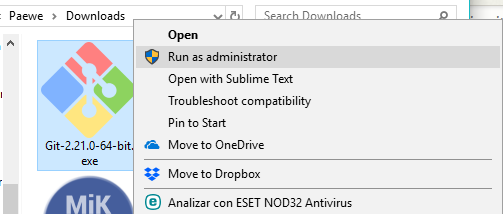
\includegraphics[scale=0.75]{./imagenes/Gitbash2.png}
\end{figure}

\begin{figure}[h!]
  \centering
  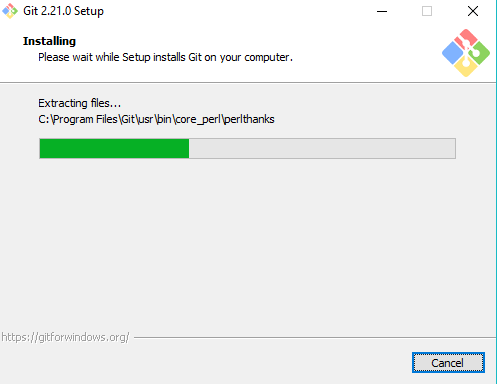
\includegraphics[scale=0.75]{./imagenes/Gitbash3.png}
\end{figure}

\clearpage

Luego de haber realizado la instalación podremos buscar el programa
llamado \textbf{Gitbash} que nos permitirá utilizar la terminal llamada
\textbf{bash} para usar git con todas sus opciones y posibilidades.

\begin{figure}[h!]
  \centering
  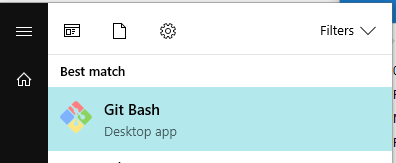
\includegraphics[scale=0.75]{./imagenes/Gitbash4.png}
\end{figure}

Una vez abierta la terminal \textbf{Bash} se procede a configurar Git tanto
el \textbf{user.name} como el \textbf{user.email}, cabe recalcar que se usará el
email de \textbf{Github} de preferencia.

\begin{figure}[h!]
  \centering
  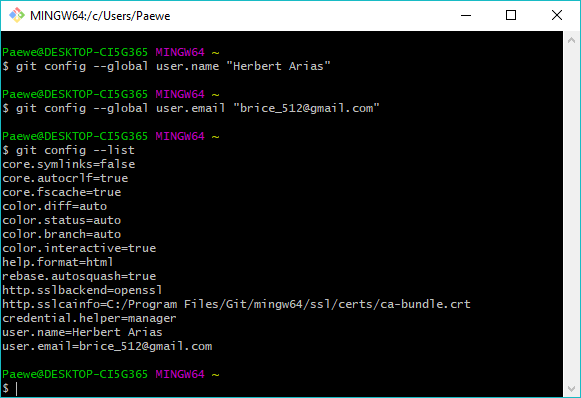
\includegraphics[scale=0.75]{./imagenes/Gitbash5.png}
\end{figure}


\section{Instalación de Texmaker}%
Por el momento dejamos Gitbash, y pasamos con la instalación de \textbf{Texmaker} y \LaTeX.
Para ello debemos descargar tres instaladores: \href{https://miktex.org/download}{Miktex},
\href{https://www.ghostscript.com/download/gsdnld.html}{Ghostscript} y
\href{http://www.xm1math.net/texmaker/download.html}{Texmaker}. Para guiarnos
podemos visualizar las figuras.

\begin{figure}[h!]
  \centering
  \subfigure[Miktex]{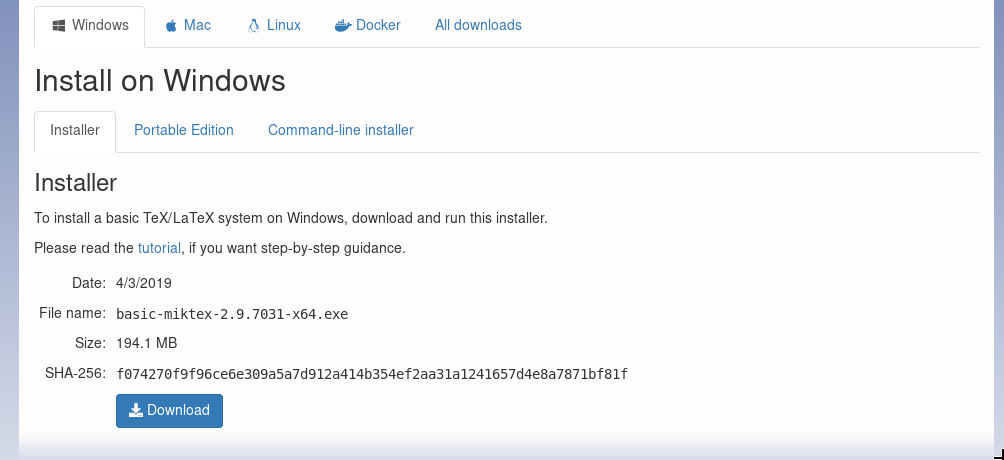
\includegraphics[scale=0.5]{./imagenes/Install_Miktex.png}}
\end{figure}

\clearpage

\begin{figure}[h!]
  \centering
  \subfigure[Ghostscript]{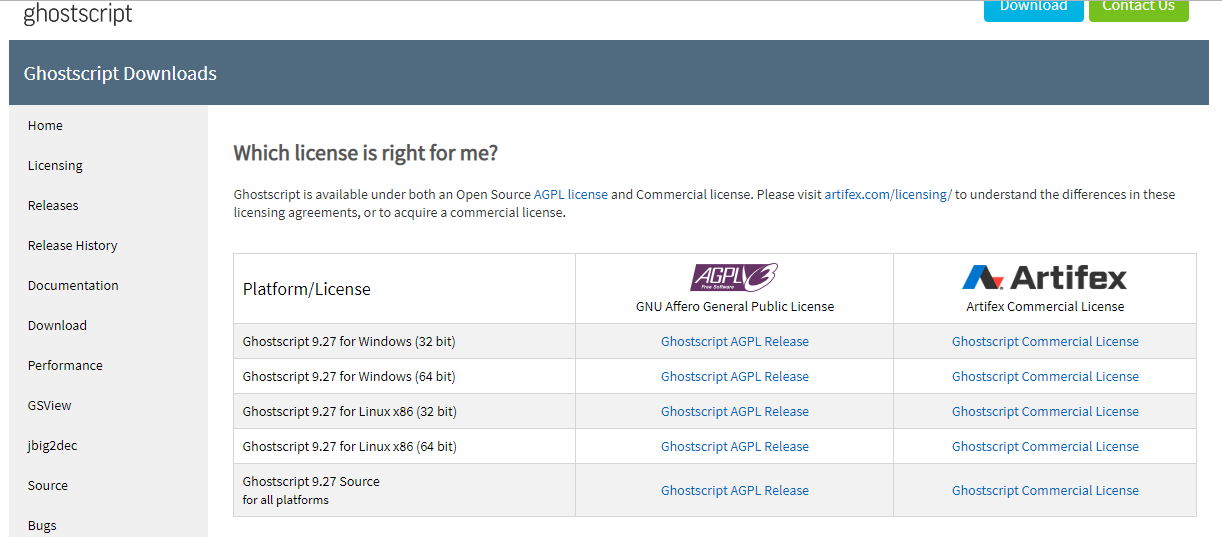
\includegraphics[scale=0.5]{./imagenes/Install_ghostscript.png}}
\end{figure}

\begin{figure}[h!]
  \centering
  \subfigure[Texmaker]{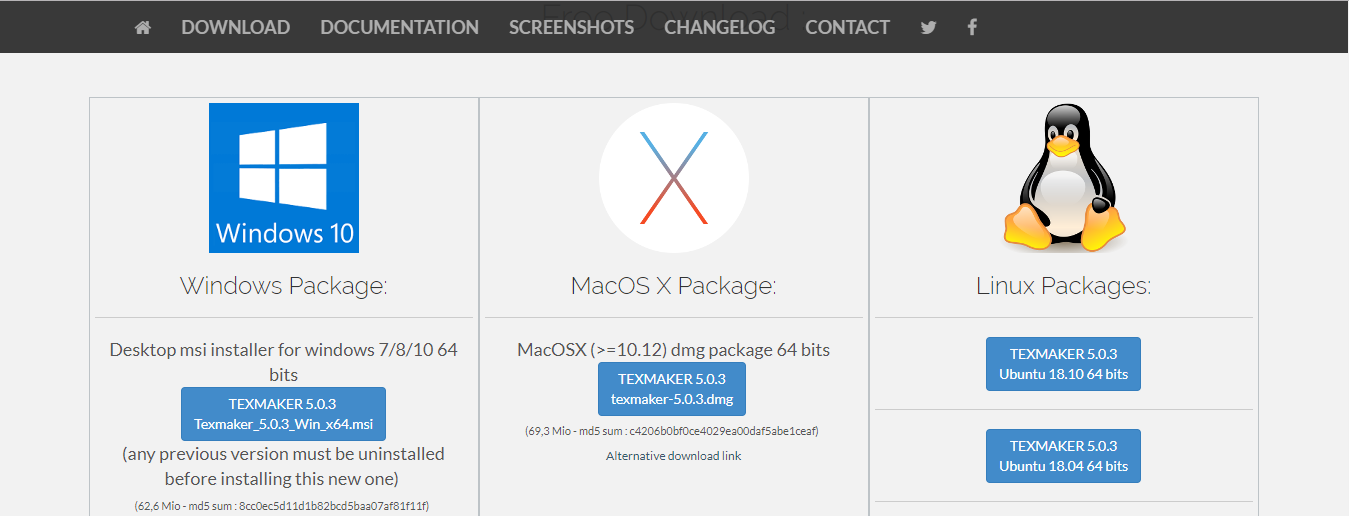
\includegraphics[scale=0.5]{./imagenes/Install_takemaker.png}}
\end{figure}


Luego de realizar las descargas tendremos tres instaladores.

\begin{figure}[h!]
  \centering
  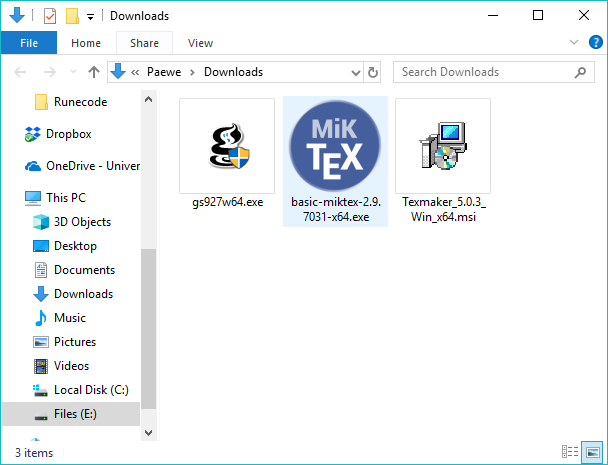
\includegraphics[scale=0.75]{./imagenes/Installers_latex.png}
\end{figure}

Tener en cuenta que al realizar la instalación de Miktex y Ghostscript se debe
guardar la ruta donde se han instalado.

\begin{figure}[h!]
  \centering
  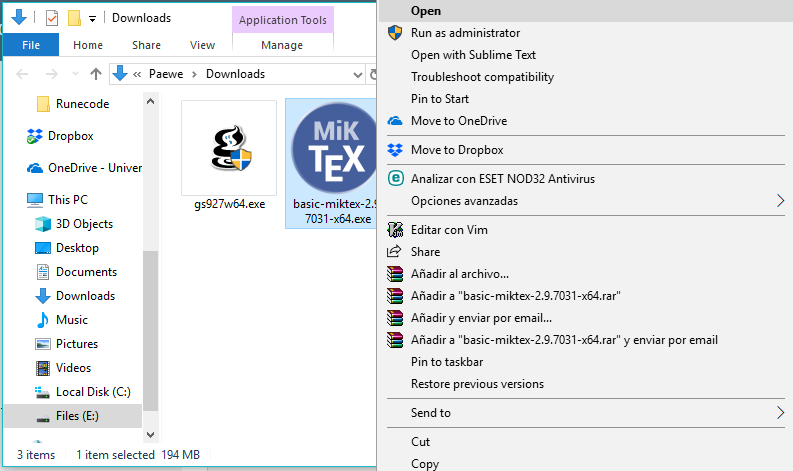
\includegraphics[scale=0.75]{./imagenes/Install_Miktex2.png}
\end{figure}

\begin{figure}[h!]
  \centering
  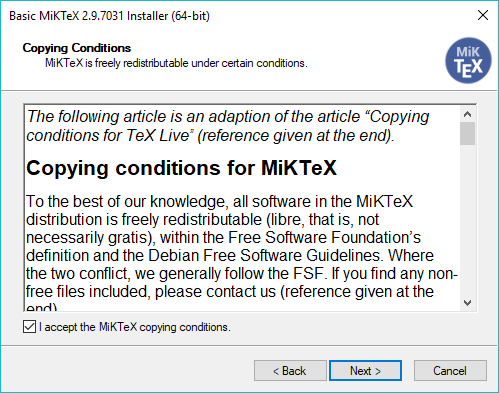
\includegraphics[scale=0.75]{./imagenes/Install_Miktex3.png}
\end{figure}

\begin{figure}[h!]
  \centering
  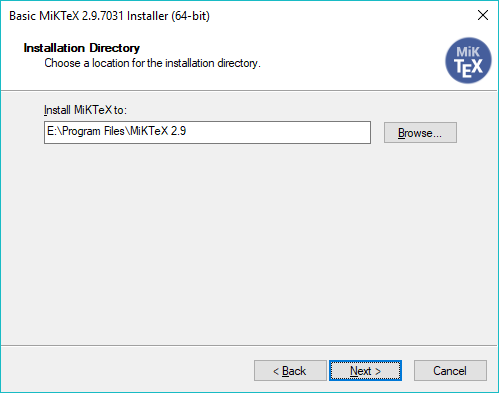
\includegraphics[scale=0.75]{./imagenes/Install_Miktex4.png}
\end{figure}

Como vemos en caso de \textbf{Miktex} se instala en la ruta
\textbf{E:{\textbackslash}Program Files{\textbackslash}MikTeX2.9}

\begin{figure}[h!]
  \centering
  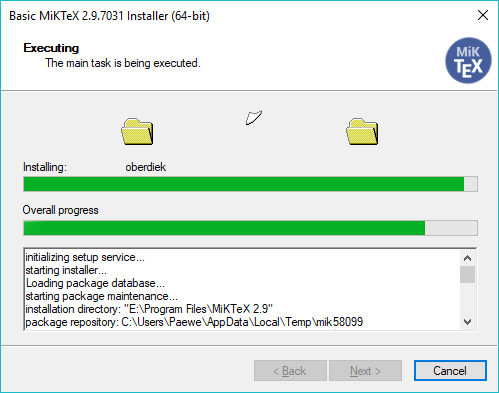
\includegraphics[scale=0.75]{./imagenes/Install_Miktex5.png}
\end{figure}

\begin{figure}[h!]
  \centering
  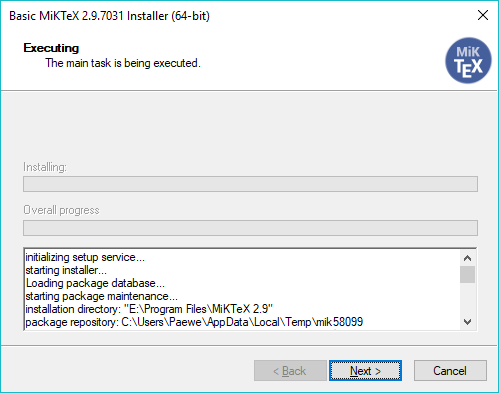
\includegraphics[scale=0.75]{./imagenes/Install_Miktex6.png}
\end{figure}
\clearpage

De igual forma la ruta en la que se ha instalado \textbf{Ghostscript} es
\textbf{C:{\textbackslash}Program Files{\textbackslash}gs{\textbackslash}gs9.27}

\begin{figure}[h!]
  \centering
  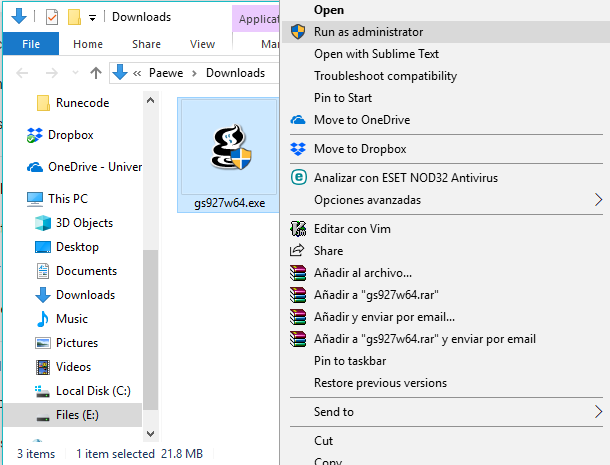
\includegraphics[scale=0.75]{./imagenes/Install_ghostscript2.png}
\end{figure}

Finalmente se instala el editor \textbf{Texmaker}.

\begin{figure}[h!]
  \centering
  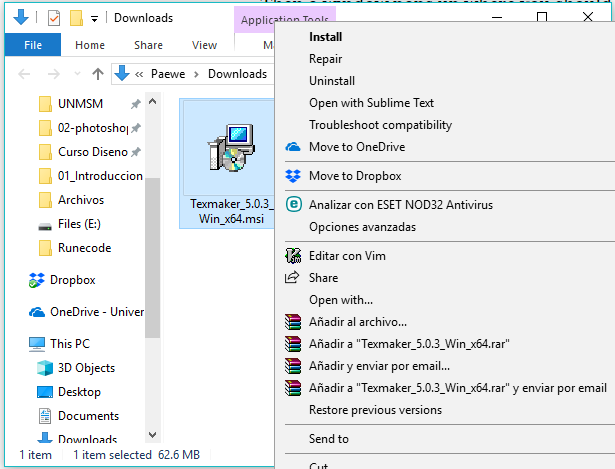
\includegraphics[scale=0.75]{./imagenes/Install_takemaker2.png}
\end{figure}
\clearpage

\begin{figure}[h!]
  \centering
  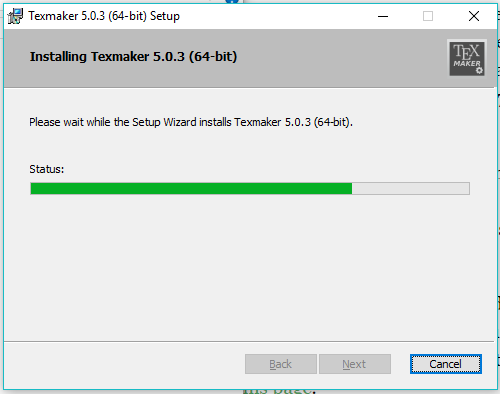
\includegraphics[scale=0.75]{./imagenes/Install_takemaker3.png}
\end{figure}

Luego de terminar la instalación procedemos con la configuración del editor
para que éste pueda compilar y previsualizar los documentos que creemos usando
\LaTeX\\

Para ello abrimos Texmaker y vamos a la ruta: \textbf{opciones / configurar texmaker}.
Nos aparece una ventana donde podremos añadir las rutas que hemos guardado
tanto de Miktex (para que compile) como de Ghostscript (para previsualizar el
documento), también se puede configurar la ruta de nuestro lector de pdf favorito que
puede ser Adobe Acrobat.

\begin{figure}[h!]
  \centering
  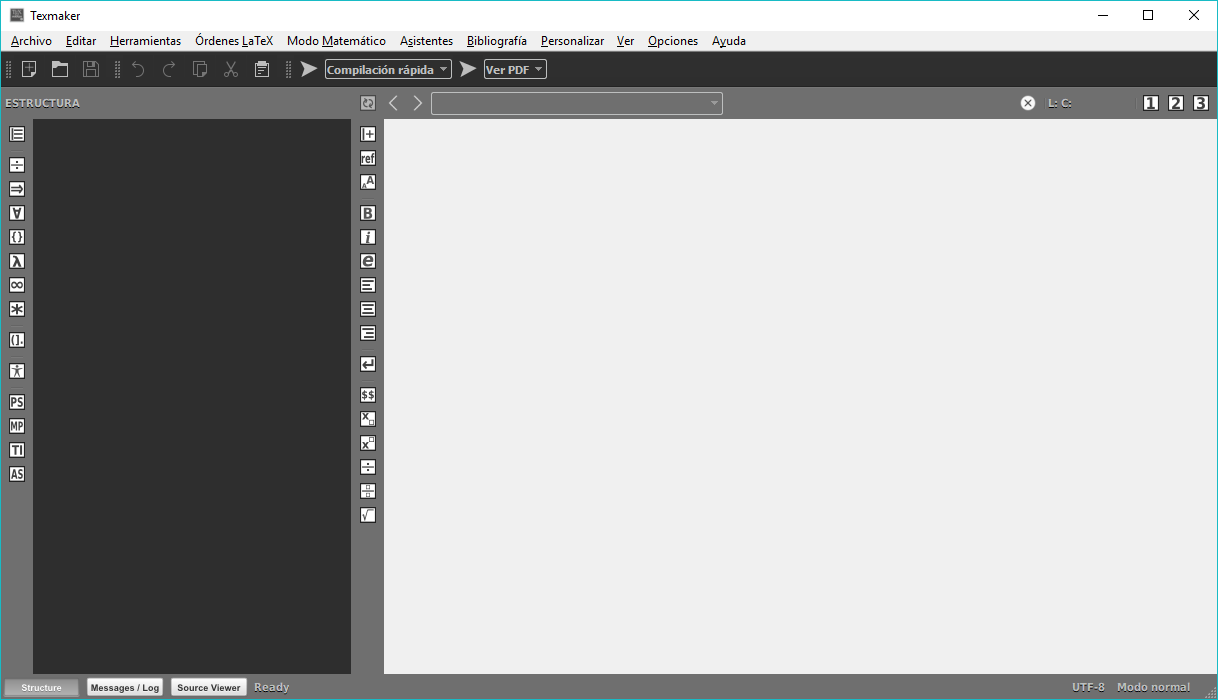
\includegraphics[scale=0.5]{./imagenes/Configuracion_texmaker.png}
\end{figure}

\begin{figure}[h!]
  \centering
  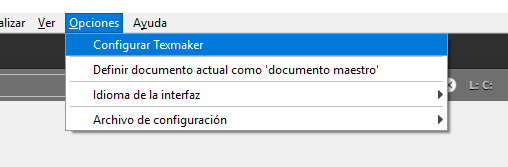
\includegraphics[scale=0.75]{./imagenes/Configuracion_texmaker2.png}
\end{figure}
\clearpage

\begin{figure}[h!]
  \centering
  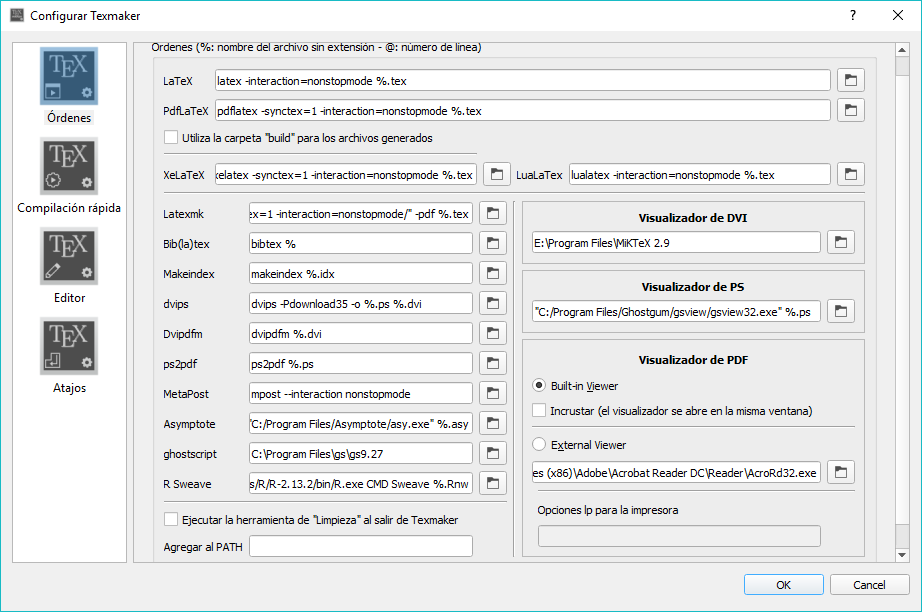
\includegraphics[scale=0.75]{./imagenes/Configuracion_texmaker3.png}
\end{figure}


\section{Instalar Python su módulo Pygments}%
Después de terminar la configuración de Texmaker, procedemos a instalar
Python 2.7, para ello nos dirigimos a su
\href{https://www.python.org/downloads/windows/}{página de descarga} y
escogemos la versión 2.7.16 que es la última versión de Python 2. En la
instalación dejamos las opciones por defecto, con esto Python estará instalado
normalmente en la ruta \textbf{C:{\textbackslash}Python27{\textbackslash}},
verifiquemos que dentro de esta carpeta se encuentra otra llamada \textbf{Scripts}.

\begin{figure}[h!]
  \centering
  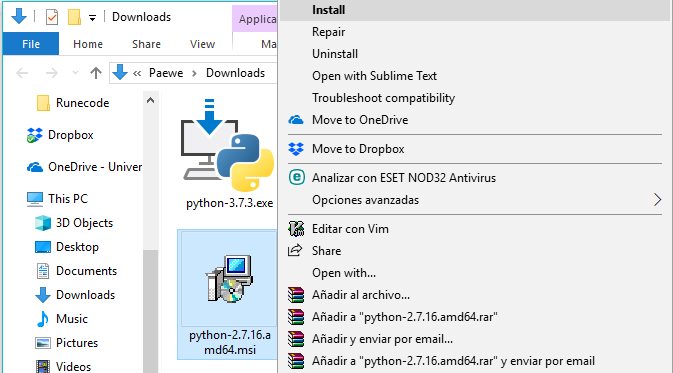
\includegraphics[scale=0.75]{./imagenes/python27_install.png}
\end{figure}

\begin{figure}[h!]
  \centering
  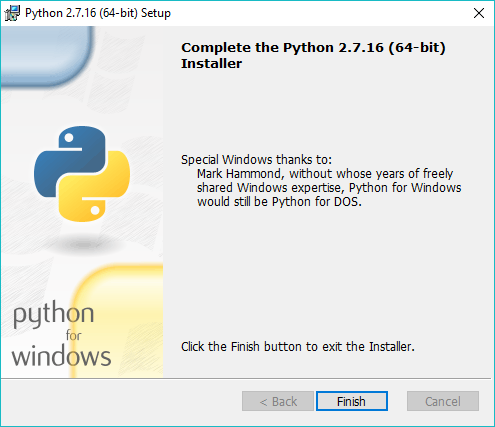
\includegraphics[scale=0.75]{./imagenes/python27_install2.png}
\end{figure}

\begin{figure}[h!]
  \centering
  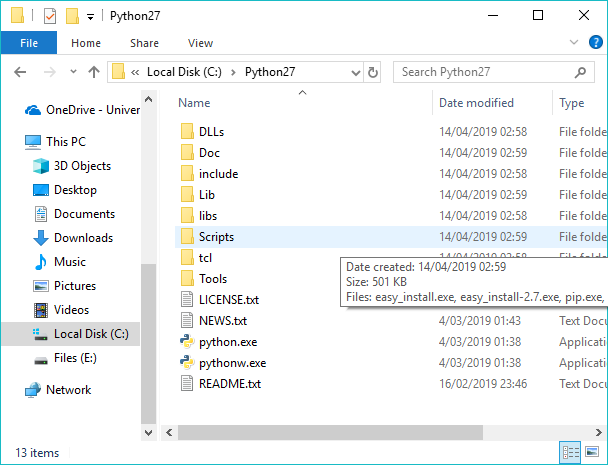
\includegraphics[scale=0.75]{./imagenes/python27_install3.png}
\end{figure}

Lo que sigue es agregar estas rutas al path de nuestro sistema, esto para poder
ejecutar python desde el cmd o desde el editor Texmaker.\\

Buscamos advanced y abrimos las \textbf{propiedades del sistema / Avanzados
(pestaña) / Variables del sistema / path / edit.} Nos saldrá una nueva ventana donde podemos
agregar la ruta donde está instalado Python y también el directorio Scripts,
tal y como observamos en las siguientes imágenes:

\begin{figure}[h!]
  \centering
  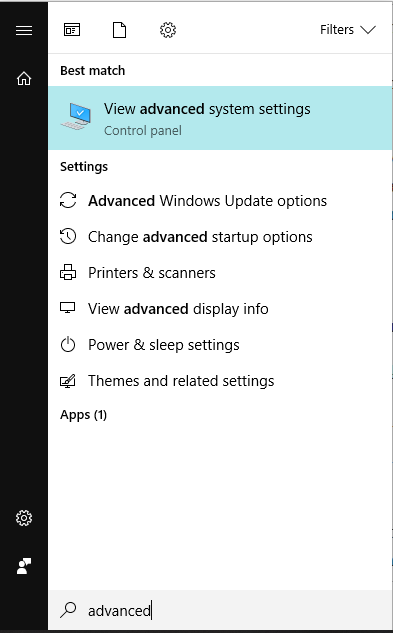
\includegraphics[scale=0.75]{./imagenes/Configurar_path.png}
\end{figure}

\begin{figure}[h!]
  \centering
  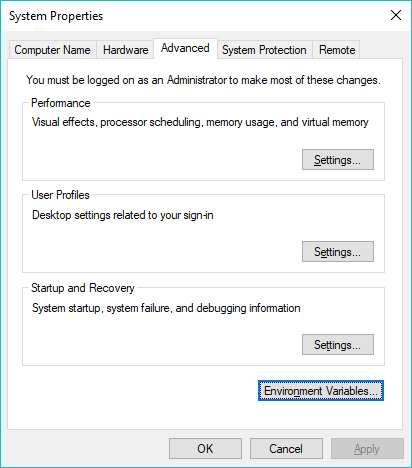
\includegraphics[scale=0.75]{./imagenes/Configurar_path2.png}
\end{figure}
\clearpage

\begin{figure}[h!]
  \centering
  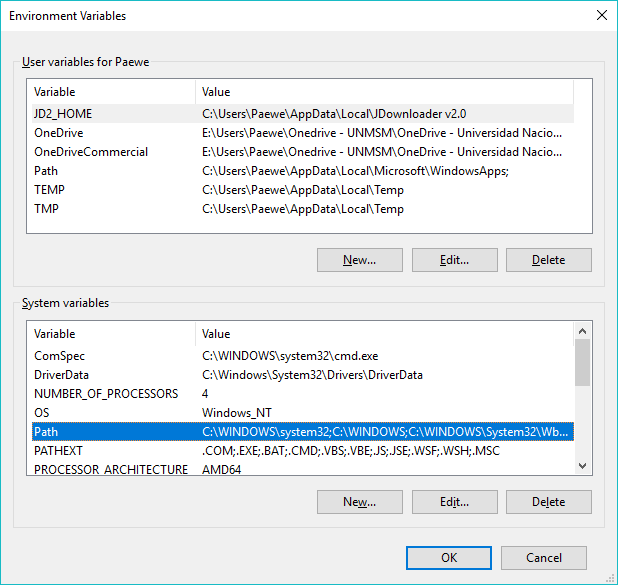
\includegraphics[scale=0.75]{./imagenes/Configurar_path3.png}
\end{figure}

\begin{figure}[h!]
  \centering
  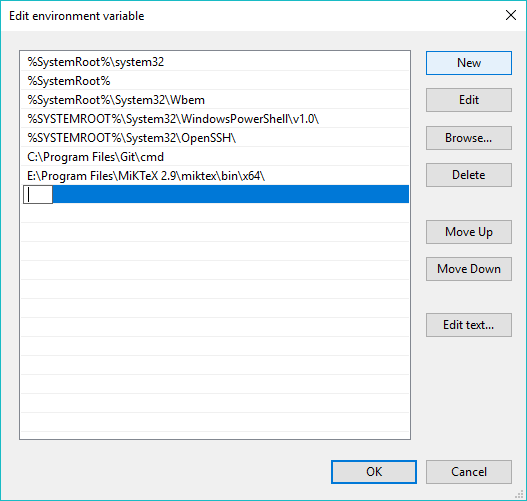
\includegraphics[scale=0.75]{./imagenes/Configurar_path4.png}
\end{figure}
\clearpage

\begin{figure}[h!]
  \centering
  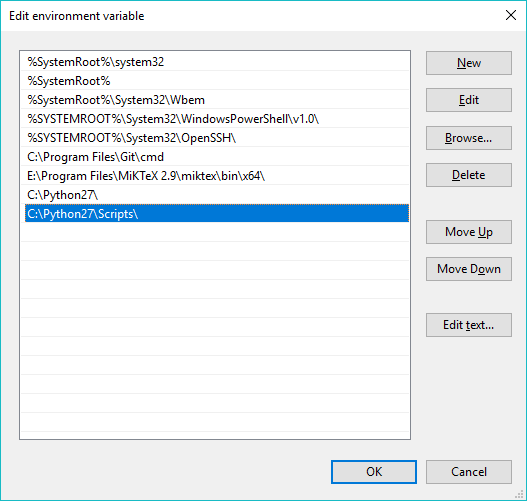
\includegraphics[scale=0.75]{./imagenes/Configurar_path5.png}
\end{figure}

Ahora podemos ejecutar cmd y verificar que tenemos instalado Python y que
podemos ejecutarlo por la terminal.
\begin{minted}[fontsize=\footnotesize, bgcolor=LightGray]
  {bash}
  python --version
\end{minted}

\begin{figure}[h!]
  \centering
  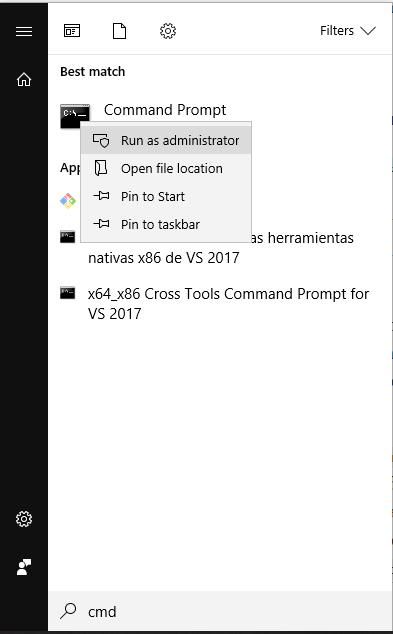
\includegraphics[scale=0.75]{./imagenes/Configurar_path6.png}
\end{figure}
\clearpage

\begin{figure}[h!]
  \centering
  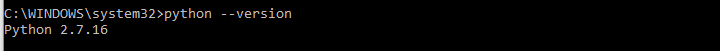
\includegraphics[scale=0.75]{./imagenes/Configurar_path7.png}
\end{figure}

Pip es un módulo de python que nos permite gestionar módulos. Podemos
actualizar pip ejecutando el siguiente comando:

\begin{minted}[fontsize=\footnotesize, bgcolor=LightGray]
  {bash}
  python -m pip install --upgrade pip setuptools wheel
\end{minted}

\begin{figure}[h!]
  \centering
  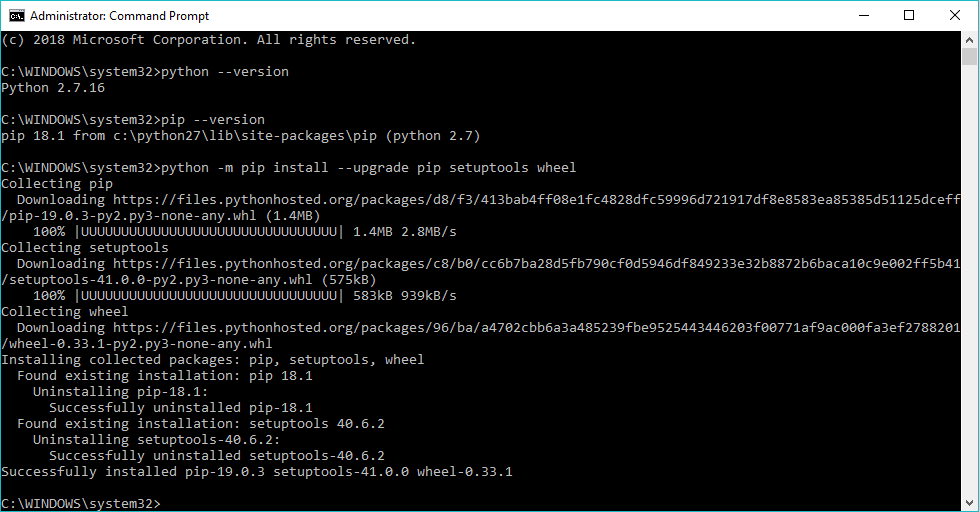
\includegraphics[scale=0.65]{./imagenes/Configurar_path8.png}
\end{figure}

Una vez actualizado pip, podemos instalar el módulo \textbf{Pygments}:

\begin{minted}[fontsize=\footnotesize, bgcolor=LightGray]
  {bash}
  pip install Pygments
\end{minted}

\begin{figure}[h!]
  \centering
  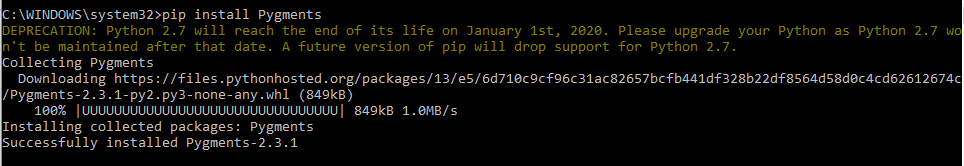
\includegraphics[scale=0.65]{./imagenes/Configurar_path9.png}
\end{figure}

El módulo \textbf{Pygments} contiene un conjunto de lexers para otorgar color a
códigos de muchos lenguajes en diferentes estilos. Para ver el conjunto lexers
(de diferenes lenguajes) que soporta el módulo podemos ejecutar el comando:

\begin{minted}[fontsize=\footnotesize, bgcolor=LightGray]
  {bash}
  pygmentize -L lexers
\end{minted}

\begin{figure}[h!]
  \centering
  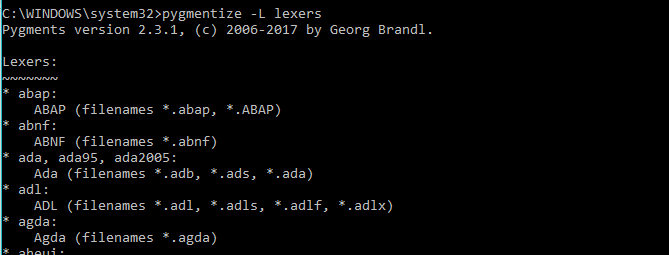
\includegraphics[scale=0.75]{./imagenes/Configurar_path10.png}
\end{figure}
\clearpage

Además podemos visualizar el conjunto de estilos disponibles:
\begin{minted}[fontsize=\footnotesize, bgcolor=LightGray]
  {bash}
  pygmentize -L styles
\end{minted}

\begin{figure}[h!]
  \centering
  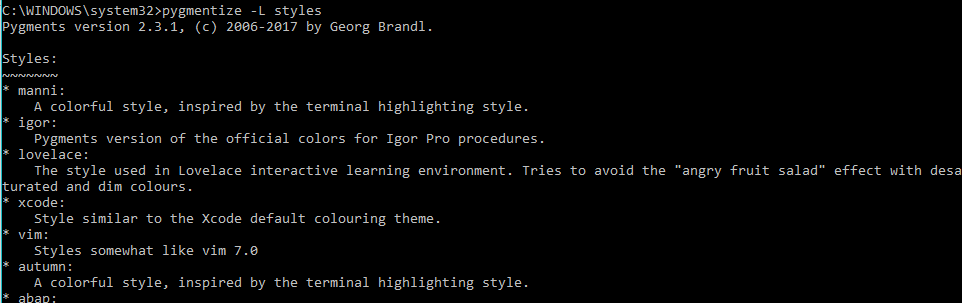
\includegraphics[scale=0.65]{./imagenes/Configurar_path11.png}
\end{figure}

Como penúltimo paso, para garantizar el correcto funcionamiento del módulo en
\textbf{Texmaker} vamos a crear un archivo en
\textbf{C:{\textbackslash}Windows{\textbackslash}pygmetize.cmd}. 
Podemos acceder a la carpeta \textbf{C:{\textbackslash}Windows{\textbackslash}}
más rápido buscando con:\textbf{\%systemroot\%}.
\begin{figure}[h!]
  \centering
  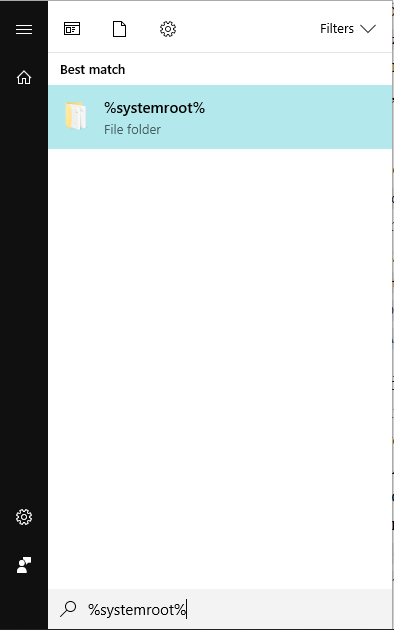
\includegraphics[scale=0.75]{./imagenes/Configurar_path12.png}
\end{figure}

En caso no poder crearlo desde el explorador de ficheros podemos abrir
\textbf{Gitbash} como administrador y dirigirnos a la
ubicación \textbf{/c/Windows/} y crear el fichero usando el
programa \textbf{touch} que viene incluido en el terminal \textbf{bash}.
\clearpage

\begin{figure}[h!]
  \centering
  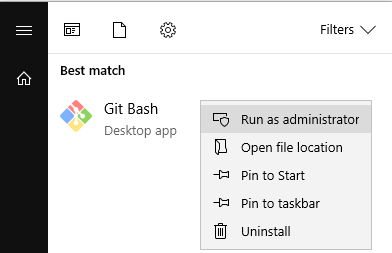
\includegraphics[scale=0.75]{./imagenes/Configurar_path13.png}
\end{figure}

\begin{figure}[h!]
  \centering
  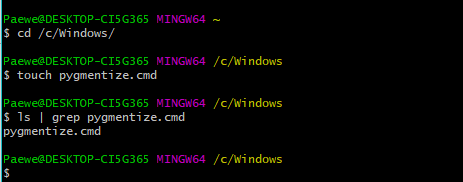
\includegraphics[scale=0.85]{./imagenes/Configurar_path14.png}
\end{figure}

Luego nos aparecerá el fichero y podremos editarlo para agregar lo siguiente:

\begin{minted}[fontsize=\footnotesize, bgcolor=LightGray]
  {bat}
  @echo off
  set PYTHONPATH=C:\Python27
  %PYTHONPATH%\python.exe %PYTHONPATH%\Scripts\pygmentize.exe %*
\end{minted}

\begin{figure}[h!]
  \centering
  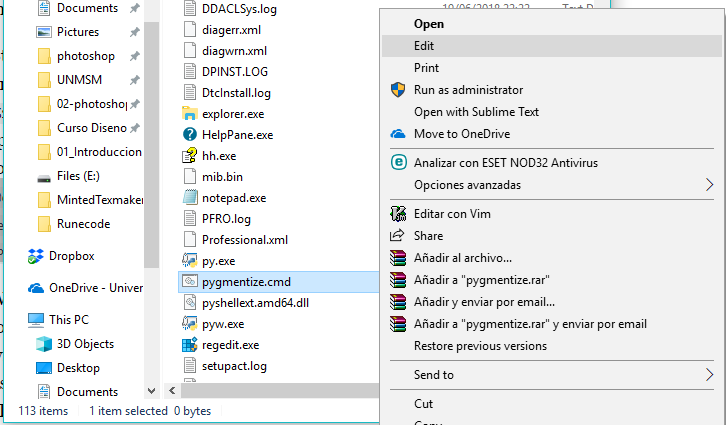
\includegraphics[scale=0.75]{./imagenes/Configurar_path15.png}
\end{figure}

\begin{figure}[h!]
  \centering
  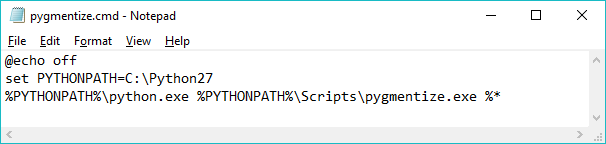
\includegraphics[scale=0.75]{./imagenes/Configurar_path16.png}
\end{figure}
\clearpage

\section{Configuración Final en Texmaker con Minted}%

Para finalizar tenemos que agregar la bandera \textbf{{-}{-}shell-escape}
en las órdenes LaTex y PdfLaTeX de \textbf{texmaker}, esto nos permitirá
compilar usando la librería minted.

\begin{figure}[h!]
  \centering
  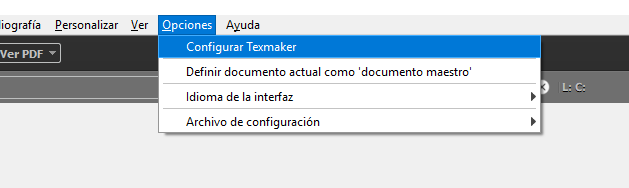
\includegraphics[scale=0.75]{./imagenes/Configurar_path17.png}
\end{figure}

\begin{figure}[h!]
  \centering
  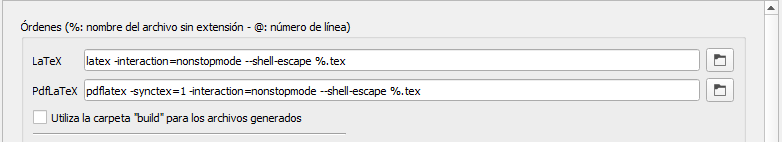
\includegraphics[scale=0.75]{./imagenes/Configurar_path18.png}
\end{figure}

\section{Manejo de repositorios en GitHub}%
Se puede manejar el repositorio de un proyecto entre varias personas de manera
muy sencilla, el creador de un repositorio puede otorgar derechos de
colaborador a cualquier usuario de GitHub, si éste usuario acepta la invitación
entonces podrá realizar \textbf{push} y subir cambios sin ninguna
restricción en el repositorio. Ésta manera de organizar un proyecto se puede
llevar a cabo cuando se tiene plena confianza en que cada colaborador realizará
los cambios más adecuados para el proyecto.\\

Primero vamos a configurar el \textbf{user.email} y \textbf{user.name} para
Git, esto ya se hizo en la primera parte de éste documento.\\

Lo que sigue es enlazar tu computadora con Github y para ello vamos a usar
el programa \textbf{Git bash}. También vamos a usar un repositorio de ejemplo
para el cual ya se ha creado una carpeta.\\

Como tip es posible acceder a Gitbash desde el explorador de archivos de
Windows con \textbf{clic derecho / Git Bash Here} que nos abrirá la terminal
con el prompt ubicado en el directorio en el que se encontraba el explorador al
momento de realizarlo.

\begin{figure}[h!]
  \centering
  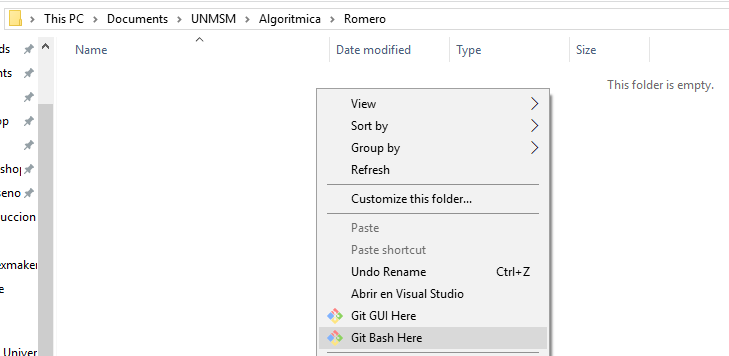
\includegraphics[scale=0.75]{./imagenes/Gitbash6.png}
\end{figure}
\clearpage

En la terminal, daremos inicio a nuestro repositorio con el siguiente comando:

\begin{minted}[fontsize=\footnotesize, bgcolor=LightGray]
  {bash}
  git init
\end{minted}

\begin{figure}[h!]
  \centering
  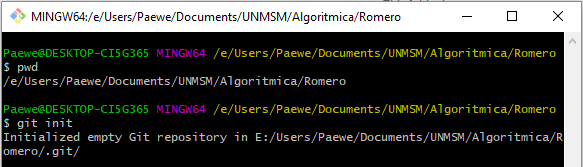
\includegraphics[scale=0.75]{./imagenes/Gitbash7.png}
\end{figure}

Github puede conectarse con tu PC de manera segura usando llaves \textbf{ssh}.
Hay dos llaves: una \textbf{privada} que no debe ser compartida y una
\textbf{pública} que se puede compartir.\\

Dicho esto vamos a generar estas llaves con el siguiente comando:

\begin{minted}[fontsize=\footnotesize, bgcolor=LightGray]
  {bash}
  ssh-keygen.exe -t rsa -b 4096 -C "tucorreo@degithub.com"
\end{minted}

Es necesario agregar como se ve en la imagen la dirección de tu correo de Gihub
con el flag \textbf{-C}.\\

Después de ejecutar este comando se generarán las dos llaves y las podemos
encontrar en la siguiente ruta: \textbf{\$HOME\$/.ssh/}, donde
\$HOME\$ suele ubicarse en \textbf{C:{\textbackslash}Documents and
Settings{\textbackslash}Usuario}

\begin{figure}[h!]
  \centering
  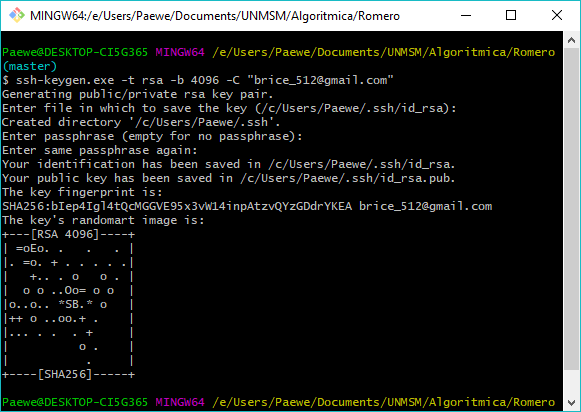
\includegraphics[scale=0.75]{./imagenes/Gitbash8.png}
\end{figure}

Se generarán dos ficheros que por defecto se llaramarán:\textbf{id\_rsa} y
\textbf{id\_rsa.pub}, siendo este último la llave pública que podemos
compartir; podemos desplegar su contenido abriéndolo con bloc de notas en la
ruta indicada o usando gitbash con el comando:

\begin{minted}[fontsize=\footnotesize, bgcolor=LightGray]
  {bash}
  cat ~/.ssh/id_rsa.pug
\end{minted}

Luego podremos copiar el contenido como se verifica en la siguiente imagen:

\begin{figure}[h!]
  \centering
  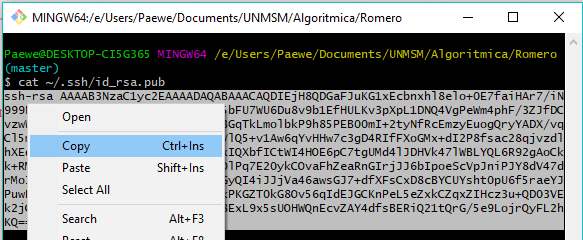
\includegraphics[scale=0.65]{./imagenes/Gitbash9.png}
\end{figure}

Pegamos la llave en Github usando la siguiente ruta: \textbf{Settings / SSH and
GPG Keys / New SSH key}, agregamos un título a la llave para identificarla y
damos clic en \textbf{Add SSH key}.

\begin{figure}[h!]
  \centering
  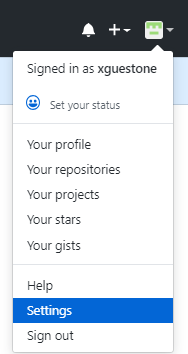
\includegraphics[scale=0.75]{./imagenes/Gitbash10.png}
\end{figure}

\begin{figure}[h!]
  \centering
  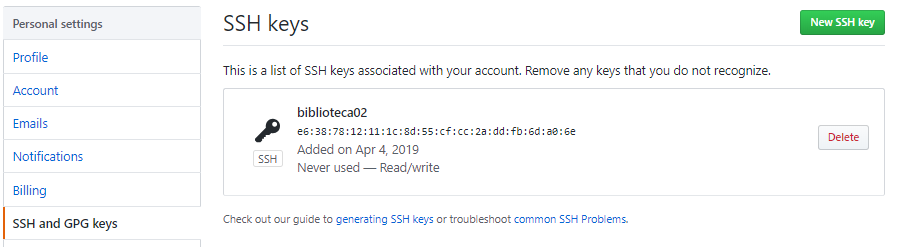
\includegraphics[scale=0.75]{./imagenes/Gitbash11.png}
\end{figure}

\begin{figure}[h!]
  \centering
  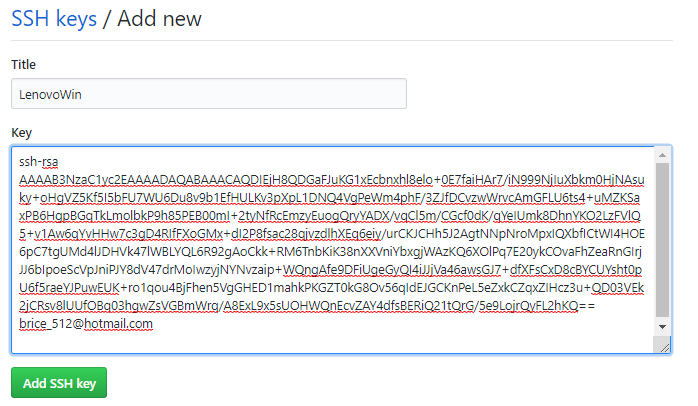
\includegraphics[scale=0.75]{./imagenes/Gitbash12.png}
\end{figure}

Con esto, nuestra computadora estará vinculada a Github y podremos subir /
bajar ficheros y repositorios a esta plataforma de manera segura.\\

Ahora proseguiremos con el repositorio \textbf{gprunecode/AlgoritRomero} al
cual ya hemos sido invitados por su creador. De ser así tendremos una
notificación que podemos ver visitando la campana en la parte superior derecha
de la página y procedemos en aceptarla.
\clearpage

\begin{figure}[h!]
  \centering
  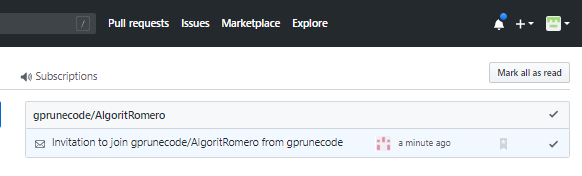
\includegraphics[scale=0.75]{./imagenes/GitHub.png}
\end{figure}

\begin{figure}[h!]
  \centering
  \includegraphics[scale=0.75]{./imagenes/GitHub2.png}
\end{figure}

\begin{figure}[h!]
  \centering
  \includegraphics[scale=0.75]{./imagenes/GitHub3.png}
\end{figure}

Luego de esto, ya seremos colaboradores y podremos subir los commits y cambios
al repositorio.\\

Ahora entramos en Github y en la sección \textbf{code} damos clic en
\textbf{Clone or download},  copiamos la dirección del repositorio de
\textbf{Clone with SSH} y lo pegamos en la terminal Git Bash de la siguiente
manera:

\begin{minted}[fontsize=\footnotesize, bgcolor=LightGray]
  {bash}
  git remote add origin git@github.com:gprunecode/AlgoritRomero.git
\end{minted}

\begin{figure}[h!]
  \centering
  \includegraphics[scale=0.5]{./imagenes/Gitbash13.png}
\end{figure}

Y luego hacemos un \textbf{fetch} al git remoto origin con el contenido del
repositorio \textbf{AlgoritRomero}.

\begin{minted}[fontsize=\footnotesize, bgcolor=LightGray]
  {bash}
  git fetch origin
\end{minted}

Veamos la siguiente imagen con el procedimiento realizado:
\clearpage

\begin{figure}[h!]
  \centering
  \includegraphics[scale=0.75]{./imagenes/Configurar_path19.png}
\end{figure}

Luego de esto ya tendremos el contenido del repositorio de Github, en nuestra
máquina, ya solo nos falta hacer un \textbf{merge} para visualizar el contenido
en nuestra carpeta.

\begin{minted}[fontsize=\footnotesize, bgcolor=LightGray]
  {bash}
  git merge origin/master
\end{minted}

\begin{figure}[h!]
  \centering
  \includegraphics[scale=0.75]{./imagenes/Gitbash14.png}
\end{figure}

\begin{figure}[h!]
  \centering
  \includegraphics[scale=0.75]{./imagenes/Gitbash15.png}
\end{figure}

Ahora vamos a buscar el fichero de extensión \textbf{tex} para compilarlo usando
Texmaker.

\begin{figure}[h!]
  \centering
  \includegraphics[scale=0.75]{./imagenes/Gitbash16.png}
\end{figure}

\begin{figure}[h!]
  \centering
  \includegraphics[scale=0.75]{./imagenes/Gitbash17.png}
\end{figure}
\clearpage

Después de realizar los cambios y demos en compilar, nos pedirá instalar
algunos paquetes:

\begin{figure}[h!]
  \centering
  \includegraphics[scale=0.75]{./imagenes/Gitbash18.png}
\end{figure}

Si realizamos algún cambio, entonces podremos dar seguimiento de los ficheros
con Git usando \textbf{status}

\begin{minted}[fontsize=\footnotesize, bgcolor=LightGray]
  {bash}
  git status
\end{minted}

Si aparecen ficheros en rojo, significa que han sido agregados, eliminados o
modificados. Estos ficheros se encuentran en nuestro \textbf{Working
Directory}, para poder agregarlos al \textbf{Staging Area} deberemos usar el
comando \textbf{add} con el nombre del fichero o con la bandera \textbf{A} que
indica agregar a todos los ficheros que han modificado su estado.

\begin{minted}[fontsize=\footnotesize, bgcolor=LightGray]
  {bash}
  git add -A
\end{minted}

Después si realizamos un \textbf{status} para verificar nuestro ficheros, los
agregados al \textbf{Staging Area} se verán de color verde listos para
consignarse como cambios en un commit.\\

Ahora podemos crear nuestro \textbf{commit}, y usando la bandera \textbf{m}
podemos agregar un comentario que describa los cambios que en él se van a
guardar.

\begin{minted}[fontsize=\footnotesize, bgcolor=LightGray]
  {bash}
  git commit -m "Mensaje descriptivo"
\end{minted}

Ya tenemos nuestro repositorio local con el commit que hemos creado y queremos
copiar este repositorio al creado en Github, para eso usamos el comando
\textbf{push}.

\begin{minted}[fontsize=\footnotesize, bgcolor=LightGray]
  {bash}
  git push origin master
\end{minted}

Esto se puede visualizar en las siguientes imágenes:

\begin{figure}[h!]
  \centering
  \includegraphics[scale=0.75]{./imagenes/Gitbash19.png}
\end{figure}

\begin{figure}[h!]
  \centering
  \includegraphics[scale=0.75]{./imagenes/Gitbash20.png}
\end{figure}

\end{document}
